\documentclass[mémoire.tex]{subfiles}
\begin{document}
\section{Approche via la théorie des singularités}\label{SINGsection}

Le lien entre l'étude des bifurcation et la théorie des 
singularités et théorie des catastrophes peut être aperçu 
dans "Stabilité structurelle et morphogenèse" de René Thom.
Ce qu'il entend par "stabilité structurelle d'un modèle 
mathématique" c'est la "persistence par rapport aux petites 
perturbations", plus précisément, pour qu'un modèle du 
monde soit prédictif, étant donné qu'il existe toujours un 
"bruit de fond" qui échappe à notre contrôle, il faut qu'il 
y soit résistant. Bien que ce soit un ouvrage plutôt 
philosophique que mathématique, les idées introduites 
furent extrêmement fécondes, si bien qu'il est impossible de 
plonger dans la théorie des singularités, ou des 
catastrophes sans croiser le nom de Thom.
\subsection{Structure algébrique des germes de fonctions lisses}
Étant donné qu'on s'intéresse uniquement au comportement des fonctions au voisinage d'un certain ensemble singulier $S$ (les points pour lesquels on ne peut appliquer le théorème des fonctions implicites) il est naturel de considérer deux fonctions comme étant "égales" si elle le sont au voisinage de $S$, nous rendons cette idée précise dans la suite 
\begin{definition}
    Soient $(X,\mathcal{T}),(Y,\mathcal{T}')$ des espaces topologiques, $S\subseteq X$ et $T\subseteq Y$
    on pose 
    \begin{align*}
        &\mathcal{G}_{0}(S,X,Y,T)=\{ f\in C^0(U,Y) | U\in\mathcal{V}_{S}^{\mathcal{T}},f(S)\subseteq T\} \\
        & \mathcal{G}_{0}(S,X,Y)=\mathcal{G}_{0}(S,X,Y,Y)
    \end{align*}
    Si de plus, on a une notion de fonction $C^k$ sur $X$ et $Y$ (par exemple, si ce sont des espaces de Banach) on définit naturellement $\mathcal{G}_k(S,X,Y,T)$ et $\mathcal{G}_k(S,X,Y)$ en imposant que les fonctions soient $C^k$ sur leur domaines. $S$ est appelé la source  et $T$ la cible
\end{definition}

\begin{definition}
    Soient $X,Y$ des espaces topologiques, $f,g\in \mathcal{G}(S,X,Y,T)$ on définit la relation d'équivalence suivante
    \begin{equation*}
        f\sim_{S} g \Leftrightarrow \exists U\in
        \mathcal{V}^{\mathcal{T}''}_{S} : f_{|_{U}}=g_{|_{U}}
    \end{equation*}
Avec $\mathcal{T}''$ la topologie induite sur l'intersection des domaines de $f$ et $g$
\end{definition}
 Bien sûr, si $f\sim_{S} g$ alors $f_{|_{S}}=g_{|_{S}}$, la définition suivante est donc licite
\begin{definition}
    Soient $X,Y$ des espaces de Banach (ou des variétés lisses), \coldef{l'espace des germes} $C^k$ est donné par
    \begin{equation*}
        \mathcal{E}(S,X,Y,T)=\mathcal{G}_{\infty}(S,X,Y,T)/\sim_{S}
    \end{equation*}
\end{definition}
Si $f\in\mathcal{E}(S,X,Y,T)$, on notera
\begin{equation*}
    f : (S,X)\rightarrow (Y,T)\text{ et }f : (S,X)\rightarrow Y\text{ si }T=Y
\end{equation*}
\begin{definition}
    Soient $f:(X,S)\rightarrow Y$ et $g:(X,S)\rightarrow Z$
    on définit 
    \begin{equation*}
       (f,g): (X,S)\rightarrow Y\times Z 
    \end{equation*}
    comme étant la classe d'équivalence de 
    \begin{equation*}
        x\mapsto (\tilde{f}(x),\tilde{g}(x))
    \end{equation*}
    où $\tilde{f}$ et $\tilde{g}$ sont des représentants de $f$ et $g$.
    Si $f:(X,S_1)\rightarrow (Y,T_1)$ et $g:(X,S_2)\rightarrow (Y,T_2)$
    alors on définit 
    \begin{equation*}
        f\times g: (X_1\times X_2,S_1\times S_2)\rightarrow 
        (Y_1\times Y_2,S_1\times S_2)
    \end{equation*}
    Comme étant la classe d'équivalence de
    \begin{equation*}
        (x_1,x_2)\mapsto (\tilde{f}(x_1),\tilde{g}(x_1))
    \end{equation*}
    Enfin, si $X'\subseteq X$ et $S'\subseteq S$, on pose $f_{|_{(S',X')}}$ est simplement la germe ayant pour représentant $\tilde{f}_{|_{X'\cap S'}}$
\end{definition}
L'opération de composition entre germes est clairement bien 
définie. Pour définir les germes de sous ensemble, on 
identifie simplement une partie $S$ à $\chi_{S}$ et 
considère la germe de fonction correspondante
\begin{definition}
    Une germe de difféomorphisme de $\mathcal{E}(\{0\},\R^n,
    \R^n)$ est un élément de $\mathcal{E}(\{0\},\R^n,\R^n,
    \{0\})$ 
    (on fixe la cible à zéro) ayant un difféomorphisme d'un 
    ouvert de $\R^n$ contenant zéro dans ses représentants. 
    Cet ensemble est noté $\mathcal{D}_n$
\end{definition}




\begin{remarque}\label{remsheaf}
    C'est un cas particulier de \coldef{faisceau}\footnote{Le lecteur familier avec la théorie des catégories ne manquera pas de remarquer qu'un faisceau est un cas particulier de foncteur contravariant de la catégorie des ouverts (dont les morphismes sont les inclusions) et la catégorie des ensembles.}
    Si $(X,\mathcal{T})$ est un espace topologique, un \coldef{faisceau} d'ensemble $\mathcal{F}$ sur $X$ est la donnée d'une famille d'ensembles $(\mathcal{F}(U))_{U\in \mathcal{T} }$ et d'une famille de fonction $(\rho^U_V: \mathcal{F}(U)\rightarrow\mathcal{F}(V))_{V\in \mathcal{T}, V\subseteq U}$ respectant les axiomes suivants :
    \begin{itemize}
        \item $\forall U\in\mathcal{T}$, $\rho^U_U = \operatorname{Id}_{\mathcal{F}(U)}$ (fonctorialité 1)
        \item $\forall U,V,W\in\mathcal{T}: U\subseteq V\subseteq W$, $\rho^V_U\circ \rho^W_V=\rho^W_U$. (fonctorialité 2)
        \item $\forall U\in\mathcal{T}, (U_i)_{i\in\mathcal{I}}\in\mathcal{T}^{\mathcal{I}}: U=\bigcup_{i\in\mathcal{I}}U_i$ si $s,t\in\mathcal{F}(U)$ sont telles que \\$ \forall i\in\mathcal{I},\rho^U_{U_i}(s)=\rho^U_{U_i}(t)$ alors $s=t$ (localité )
        \item $\forall U\in\mathcal{T}, (U_i)_{i\in\mathcal{I}}\in\mathcal{T}^{\mathcal{I}}: U=\bigcup_{i\in\mathcal{I}}U_i$, si $s_i\in\mathcal{F}(U_i)$ et si $\rho^U_{U_i\cap U_j}(s_j)=\rho^U_{U_i\cap U_j}(s_i)$ alors $\exists s\in\mathcal{F}(U)$ telle que $\forall i\in\mathcal{I},\rho^U_{U_i}(s)=s_i$ (recollage)
    \end{itemize}
    Les deux axiomes sont des axiomes purement structurels. Les deux autres permettent de capturer les propriétés désirées. Ainsi,si $Y,X$ sont des variétés lisses alors $C^{\infty}(\cdot,Y): U\mapsto C^{\infty}(U,Y)$ est un faisceau. Et si on définit enfin la \coldef{germe} d'un faisceau en un sous-ensemble $S\supseteq X$ comme étant
    \begin{equation*}
        \mathcal{F}_S=\varinjlim_{U \supseteq S} F(U)
    \end{equation*}
    alors
    \begin{equation*}
        \mathcal{E}(S,X,Y)=C^{\infty}(\cdot,Y)_{S}
    \end{equation*} 
\end{remarque}
Dans la suite, $N$ sera une variété lisse de dimension $n$. On pose $\mathcal{E}(N)_S
=\mathcal{E}_S(S,N,\R)$, si le contexte est clair, on notera $\mathcal{E}_S$. On 
remarque que les opérations de multiplication et d'addition 
passent au quotient, ce qui en fait un 
anneau commutatif. On remarque également que l'évaluation 
en $0$ et la dérivée passent aussi au quotient. Dans les prochaines pages, on étudie cet anneau ainsi que les modules qu'on peut construire dessus. Pour ce faire, nous adaptons le travail de John Mather \cite{Mather1968vol3}
\begin{remarque}
    Des notions similaires existent en dimension infinie. 
    C'est assez marginal car en pratique, l'approche par 
    théorie des singularités suppose qu'on a effectué la 
    réduction de  Lyapunov–Schmidt.
\end{remarque}




On rappelle la notion d'anneau local 
\begin{definition}
    Un anneau commutatif $R$ est local s'il a un unique idéal maximal. Il est semi local s'il a un nombre fini d'idéaux maximaux
\end{definition}

\begin{proposition}
    Si $S=\left\{s\right\}$ est un singleton,
    l'ensemble $\mathcal{M}_S=\mathcal{E}_s(s,N,\R,0)$ est l'unique idéal maximal de $\mathcal{E}_s$. En particulier, $\mathcal{E}_{s}(N)$ est un anneau local.
\end{proposition}
\begin{preuve}
Il suffit d'observer que si $f\in\mathcal{E}_S
\setminus\mathcal{M}_s$, alors il est  inversible. En effet, 
si $\tilde{f}\in f$ alors $1/\tilde{f}$ est défini sur un 
voisinage de $s$ et $g=[1/\tilde{f}]_{\sim_s}$ est 
l'inverse de $f$
\end{preuve}
Le lemme suivant montre qu'on peut se ramener au cas ou $S$ est connexe
\begin{proposition}\label{décomposition}
    Soit $N$ une variété lisse $S\subseteq N$
    \begin{equation*}
        S=\bigcup_{j=1}^p S_j\text{ et } \bar{S_i}\cap 
        \bar{S_{i'}}=\emptyset\text{ si } i\neq i'\Rightarrow \mathcal{E}_S\cong \prod_{j=1}^p \mathcal{E}_{S_i}(N)\text{ et }\mathcal{M}_S=\prod_{j=1}^p \mathcal{M}_{S_j}(N)
    \end{equation*}
\end{proposition}
\begin{preuve}
    Souvenez vous qu'on suppose que les variétés sont des espaces topologiques séparés, il existe donc $U_1,\cdots,U_p$ des voisinages de $S_1,\cdots,S_p$. Soit maintenant une germe $f\in\mathcal{E}_S$, c'est la classe d’équivalence d'une fonction $\tilde{f}$ défini sur un voisinage $V'$ de $S$, on pose alors $V'=\bigcup_{j=1}^p V_j=\bigcup_{j=1}^p V\cap Uj$. Bien sûr, 
    $\tilde{f}_{|_{V'}}\sim_{S} \tilde{f}$
    et donc on vérifie facilement que 
    \begin{equation*}
        \Phi : \mathcal{E}_S\rightarrow \prod_{j=1}^p 
        \mathcal{E}_{S_i}(N), [f]_S\mapsto ([f|_{V_1}]_{S_1},\cdots [f|_{V_p}]_{S_p} )
    \end{equation*}
    est un isomorphisme d'anneau. La décomposition de l'idéal $\mathcal{M}_S$ en découle immédiatement.
\end{preuve}
\begin{corollaire}
    Si $S$ est fini, $\mathcal{E}_S$ est un anneau semi-local.
\end{corollaire}

\begin{remarque}
    Dans la littérature (\cite{damon1984unfolding},\cite{montaldi2021sbc}) il est assez courant qu'on se restreigne à l'étude de germes de \coldef{points}. Dans ce cas, on peut "oublier" le fait qu'on travaille sur une variété et simplement supposer qu'on est dans $\R^n$. Ca n'est bien sûr pas le cas en général. Par exemple, si $S$ est une sous variété de dimension $\geq 1$, on voit immédiatement que $\mathcal{E}_S$ n'est pas un anneau local, ou même semi-local. Les choses deviennent incroyablement plus compliquées si on s'intéresse aux germes de sous variétés (ou de sous ensembles arbitraires), nous n'exploreront donc pas cette direction, le lecteur intéressé peut par exemple consulter [SOURCE]
\end{remarque}

Dans la suite, si $R$ est anneau, on notera $R^r[x_1,\cdots,x_n]$ le polynômes de degré $r$ en $x_1,\cdots,x_n$, $R[x_1,\cdots,x_n]_r$ les polynômes homogènes de degré $r$.
Le lemme suivant mobilise le fait que $N$ est de dimension finie, et nous permettra de décomposer $\mathcal{M}_N(S)$


\begin{proposition}(Lemme d'Hadamard)\label{Hadamard}
Soit $x\in N$, $(\tilde{x}_1,\cdots,\tilde{x}_n)$ un système de coordonnées 
locales qui s'annule en $x$. Considérons l'idéal $I(k,r)\subseteq \mathcal{E}_x(N)$ 
des germes ayant un représentant $\tilde{f}: U\rightarrow \R$ 
dont les dérivées d'ordre $<r$ s'annulent sur $ 
U\cap(\tilde{x}_1,\cdots,\tilde{x}_k)^{-1}(0)$ et $x_1,\cdots,x_n$ les germes  ayant pour représentants $\tilde{x}_1,\cdots,\tilde{x}_n$
    \begin{equation*}
     \rangle \mathbb{Z}[x_1,\cdots,x_k]_{r} \langle_{\mathcal{E}_x(N)}=I(k,r)
    \end{equation*}
\end{proposition}
\begin{preuve}
Il est clair que $\mathbb{Z}[x_1,\cdots,x_k]_{r}\subseteq I(k,r)$. Nous montrons l'autre inclusion en procédant par récurrence. Soit alors $f\in I(k,r)$, pour $1\leq i\leq k$, on pose 
\begin{equation*}
    \tilde{f}_i(\tilde{x_1},\cdots,\tilde{x_n})=\int_{0}^
    {1}  D_i \tilde{f}(0,\cdots,0,t\tilde{x}_i,\tilde{x}_{i
    +1},\cdots,\tilde{x}_n)dt
\end{equation*}
si $f_i=[\tilde{f}_i]$, on a alors
\begin{equation*}
    f=\sum_{i=1}^{k}x_i f_i
\end{equation*}
ce qui nous permet de conclure quand $r=1$. Maintenant, si 
$f\in I(k,r)$, alors $f_i\in I(k,r-1)$. Par hypothèse de 
récurrence, $f_i\in  \mathbb{Z}[x_1,\cdots,x_k]_{r-1}$, et 
$f=\sum_{i=1}^{n}x_i f_i$, on conclut.
\end{preuve}

Ce résultat nous permet d'affirmer que 
\begin{equation*}
    \mathcal{M}_x(N)=\rangle x_1,\cdots,x_n \langle_
    {\mathcal{E}_S}
\end{equation*}
et que $\mathcal{M}_x(N)^r$ est exactement égale aux germes 
dont les dérivées d'ordres $<r$ sont nulles en $0$.\\
Si $R$ est un  anneau, on note $R[[X_1,\cdots,X_n]]$ 
l'ensemble 
des séries formelles à $n$ variables\footnote{ On pourrait 
tout à fait avoir un nombre infini de variable}. Rappelons 
qu'une série formelle peut être vue comme une fonction qui 
à un  
multi-indice $\alpha\in\mathbb{N}^n$ associe un  élément 
$c_{\alpha}\in R$, appelé le coefficient de $X^{\alpha}$, et 
on représente $f\in R[[X_1,\cdots,X_n]]$ de la façon 
suivante
\begin{equation*}
    f=\sum_{\alpha\in\mathbb{N}^n} c_{\alpha}X^{\alpha}\text
    { avec } c_{\alpha}=f(\alpha)
\end{equation*}
On munit $R[[X_1,\cdots,X_n]]$ d'une structure d'anneau via 
\begin{align*}
    &\sum_{\alpha\in\mathbb{N}^n} c_{\alpha}X^{\alpha}+\sum_
    {\alpha\in\mathbb{N}^n} b_{\alpha}X^{\alpha}= \sum_
    {\alpha\in\mathbb{N}^n}(c_{\alpha}+b_{\alpha})X^{\alpha}
    \\
    &(\sum_{\alpha\in\mathbb{N}^n} c_{\alpha}X^{\alpha})
    \cdot (\sum_{\alpha\in\mathbb{N}^n} b_{\beta}X^{\beta})
    =\sum_{\alpha,\beta\in\mathbb{N}^n}c_{\alpha}b_{\beta}X^
    {\alpha+\beta}
\end{align*}
On Rappelle également que ce nouvel anneau hérite de 
certaines propriétés de l'anneau $R$, en particulier si $R$ 
est local, $R[[X_1,\cdots,X_n]]$ l'est aussi, et l'unique 
idéal maximal $\mathcal{M}$ est l'ensemble des séries dont 
le terme constant est dans $\mathcal{M}$.

\begin{corollaire}\label{Isopoly}
    Avec les notations du résultat précédent, 
    \begin{equation*}
        \mathcal{E}_x(N)/\mathcal{M}_x(N)^r\cong \mathbb{R}
        [[x_1,\cdots,x_n]]/\mathcal{M}^r
    \end{equation*}
    avec $\mathcal{M}$ l'unique idéal maximal de $\mathbb{R}
    [[x_1,\cdots,x_n]]$
\end{corollaire}
\begin{preuve}
    Considérons 
    \begin{equation*}
        J_{x}^{r-1}: \mathcal{E}_x(N)\rightarrow \R[[x_1,\cdots,x_n]]/\mathcal{M}^r
    \end{equation*}
    qui à $f$ associe son développement de Taylor à l'ordre 
    $r-1$, via \ref{Hadamard}, on sait que $\ker J_{x}^{r-1}
    =\mathcal{M}_x(N)^r$ en $x$, et il est évidemment surjectif. On conclut en appliquant le premier théorème d'isomorphisme.
\end{preuve}
On va désormais s'intéresser aux modules sur l'anneau $\mathcal{E}_S$ avec $S$ fini, on rappelle que 

\begin{definition}
    Soit $R$ un anneau, un $R$-module\footnote{Attention, ici on suppose tous les modules unitaires, c'est pas le cas de tous les auteurs. Ainsi, certains ne supposent pas la quatrième condition vraie pour tous les anneaux} à gauche est la donnée d'un groupe abélien $G$ est d'une opération "multiplier par un scalaire" $\cdot:R\times G\rightarrow G$ qui respecte les mêmes axiomes que pour un espace vectoriel, i.e, $\forall r,s\in R,x,y\in G$
    \begin{align*}
        &r\cdot(x+_{G}y)= r\cdot x+_{G}r\cdot y\\
        &(r+_{R} s)\cdot x = r\cdot x+_{G} s\cdot x\\
        &(r\cdot_{R}s)\cdot x=r\cdot(s\cdot x)\\
        &1_{R}\cdot x =x
    \end{align*}
\end{definition}

\begin{definition}
    Un module est dit \coldef{libre} s'il possède une base. Un module est \coldef{finiment généré} s'il possède une partie génératrice finie. Enfin, un module libre est à \coldef{rang constant} si toutes les bases ont le même nombre d'éléments
\end{definition}
Contrairement aux espaces vectoriels, les modules ne sont pas forcément libres
\begin{exemple}
    Considérons par exemple
    $S=\left\{ (x,y,z)\in\R^3| 
    x=0,z=0\right\}$, $\mathcal
    {E}_S(\R^3)$. L'idéal $I_S$ 
    constitué des fonctions qui s'annulent sur $S$ est bien 
    sûr un $\mathcal{E}_S(\R^3)$-module. Par \ref{Hadamard}, on a $I_S= \rangle x,z \langle$. Mais on peut écrire 
    \begin{equation*}
        z\cdot y + (-y)\cdot z= 0
    \end{equation*}
    et les  germes fonctions $x$ et $-y$ ne sont pas nulles sur $\mathcal{E}_S$. Il est donc impossible d'avoir une base
\end{exemple}

On peut aussi avoir la situation où $r\cdot x=0$ avec $r$ 
et $x$ non nuls, c'est ce qu'on appelle un module à \coldef
{torsion}. La notion d'homomorphisme de module est la même 
que celle d'application linéaire.
Nous rappelons (sans preuve) le lemme de Nakayama, qui est 
central dans l'étude des $\mathcal{E}_S$-modules 

\begin{theobox}{Lemme de Nakayama}{}\label{Nakayama}
    Soit $R$ un anneau commutatif, $u:E\rightarrow F$ un homomorphisme de $R$-modules, $I$ un idéal de $R$ tel que $1_{R}+z$ est inversible pour tout $z\in I$.
    Si $F$ est finiment généré, on a 
    \begin{equation*}
        u(E)+ IF=F\Rightarrow u(E)=F
    \end{equation*}
\end{theobox}
par $IF$ on entend l'ensemble des sommes finies d’éléments $if$ où $i\in I$, $f\in F$.\\
On aura également besoin de ce petit corollaire
\begin{corollaire}\label{corrNakayama}
    Soit $M$ est un $R$-module finiment généré avec $R$ un anneau local d'idéal maximal $\mathcal{M}$. Si $[m_1],\cdots,[m_k]$ génèrent $M/\mathcal{M}M$, alors 
    $m_1,\cdots,m_k$ génèrent $M$.
\end{corollaire}
\begin{definition}
    Si $M$ est un $R$-module et $N$ un sous module, on définit le module quotient de la façon habituelle:
    \begin{equation*}
        M/N=\left\{ m+N | m\in M \right\}
    \end{equation*}
\end{definition}
 Rappelons également que le "troisième théorème 
 d'isomorphisme" ou "théorème C" est vrai pour les modules. 
 On a donc, pour un module $M$, et $T$, $S$ des sous 
 modules tels que $T\subseteq S\subseteq M$,
\begin{equation*}
    (M/T)/(S/T)\cong M/S
\end{equation*}

Vous remarquerez qu'on a pas mis 
d'hypothèses pour le sous 
module (contrairement aux 
quotient de groupes). C'est 
parce 
qu'on en a pas besoin pour que les opérations soient bien 
définies ! Ainsi, on vérifie facilement que $M/N$ est bien 
un sous module. Notez que le quotient d'un $\mathcal{E}_S
$-module par un sous module est, en 
particulier, un espace 
vectoriel sur $\R$ (en identifiant  les 
germes constantes à 
leurs constantes). Donc dans la suite, $\dim_{\R} (M/N)$ 
signifiera la dimension de $M/N$ en tant que $\R$-vectoriel.
\\

Les résultats suivants nous permettent de contrôler le nombre de 
générateurs d'un sous module d'un $\mathcal{E}_S$-module 
finiment généré
\begin{lemme}\label{Lemme inclusion}
    Soient $S$ un ensemble fini, $M$ un 
    $\mathcal{E}_S$-module finiment généré et $V$ un 
    sous module de $M$, on a 
    \begin{equation*}
        \dim_{\R}( M/(\mathcal{M}_S^{l+1}M+V))\leq 
        l\Rightarrow \mathcal{M}_S^{l}M\subseteq V
    \end{equation*}
\end{lemme}
\begin{preuve}
    Par le théorème C, il vient, en posant $M'=M/V$
    \begin{equation*}
        \dim_{\R}( M/(\mathcal{M}_S^{l+1}M+V))=\dim_{\R}
        ( M'/(\mathcal{M}_S^{l+1}M'))\leq l
    \end{equation*}
    Remarquez qu'on a 
    \begin{equation*}
        M'\supseteq M'\mathcal{M}_S\supseteq M'\mathcal{M}^2_S(N)\supseteq \cdots \supseteq M'\mathcal{M}^{l+1}_S(N)
    \end{equation*}
    et donc 
    \begin{equation*}
        0=\dim_{\R} M'/M'\leq \dim_{\R} M'/( M'\mathcal{M}_S)\leq\cdots \leq  \dim_\R M'/(M'\mathcal{M}_S^{l+1})\leq l
    \end{equation*}
    et donc il existe $0\leq k \leq l$ tel que 
    \begin{equation*}
        \mathcal{M}_S^{k+1}M'=\mathcal{M}_S^{k}M'
    \end{equation*}
    On applique alors \ref{Nakayama} avec $E=0$, $R=\mathcal{E}_S$, $I=\mathcal{M}_S$ et $F=\mathcal{M}_S(M)^kM'$, ce qui permet d'affirmer que $\mathcal{M}_S^k M'=\mathcal{M}_S^k (M/V)=0$ ce qui permet de conclure.
\end{preuve}



\begin{proposition}
    Dans les hypothèses du lemme précédent, si $S=\left\{s\right\}$ alors $M'$ est finiment généré (en tant que $\mathcal{E}_S$-module) 
    il existe un ensemble de générateurs ayant au plus $m$$ 
    {n+l}\choose {l}$ éléments, où $m$ est la taille du plus petit ensemble de générateurs de $M$
\end{proposition}

\begin{preuve}
    Du fait que 
    $\mathcal{M}_S^lM$ est finiment généré et 
    $M/(\mathcal{M}_S^lM)$ est de dimension finie (via 
    \ref{Isopoly}), $\mathcal{M}_S^{l}M+V$ est finiment 
    généré et, via le résultat précédent, 
    $V=\mathcal{M}_S^{l}M+V$ donc $V$ est finiment généré. 
    Via le corollaire \ref{corrNakayama}, un ensemble de 
    générateurs de   $V/\mathcal{M}_SV$ donne un ensemble de générateurs de $V$. Il vient alors 
    \begin{equation*}
        \dim_{\R} V/\mathcal{M}_SV\underset{\text{via \ref{Lemme inclusion}}}{\leq}\dim_{\R} V/\mathcal{M}^{l+1}_SM\leq \dim_{\R} M/\mathcal{M}^{l+1}_SM\underset{\text{via} \ref{Isopoly}}{\leq}  m{n+l\choose l}
    \end{equation*}
\end{preuve}

\begin{remarque}
    On vient de montrer que tout $\mathcal{E}_S$-module
    finiment généré avec $S=\left\{s\right\}$ est un module \coldef{noethérien}, i.e un module dont tous les sous-modules sont finiment générés
\end{remarque}


\begin{corollaire}
    Tout $\mathcal{E}_S$-module $M$ finiment généré, avec $S$ fini, est un module Noetherien
\end{corollaire}

Soient $P$ une variété et $y\in P$,
on considère alors les projections 
$\pi:((y,0),P\times \R)\rightarrow P$ et $t:((y,0),
P\times \R)\rightarrow \R$. Remarquez que l'espace des germes $\mathcal{E}(y,P,\R^m)$ est isomorphe à  $\mathcal{E}_{y}(P)^m$, on pose alors

\begin{equation*}
    R_{\cdot}:\mathcal{E}_y(P)^m\rightarrow \mathcal{E}_{(y,0)}(P\times \R),u\mapsto \sum_{i=1}^{m}(u_i\circ \pi)t^{m-i}
\end{equation*}

et 

\begin{equation*}
    \Gamma_{\cdot}:\mathcal{E}_y(P)^m\rightarrow \mathcal{E}_{(y,0)}(P\times \R),u\mapsto t^m+R_u
\end{equation*}

Le résultat suivant est une conséquence du \colprop{théorème 
de division de Mather}, la preuve étant assez lourde et 
calculatoire, il est simplement rappelé

\begin{lemme}\label{DivMather}
Soient $g\in\mathcal{E}_{(y,0)}(P\times \R)$ et 
$u\in\mathcal{E}_y(P)^m$, il existe $h\in\mathcal{E}_y(P)
^m$ telle que
\begin{equation*}
    g=\Gamma_u q +R_h
\end{equation*}
\end{lemme}
\begin{definition}
    $f\in\mathcal{E}_{(y,0)}(P\times\R)$ est dite $m$-régulière si la germe $f|_{(y\times \R, (y,0) )}$ (identifiée à un élément de $\mathcal{E}_0(\R)$ ) si ses dérivées d'ordre $0\leq i < m$ sont nulle en l'origine, mais pas la dérivée d'ordre $m$.
\end{definition}

Le théorème suivant montre que le "terme de reste" du lemme précédent disparaît si $f$ est régulière

\begin{theorem}
    Si $f\in\mathcal{E}_{(y,0)}(P\times\R)$ $m$-régulière, alors il existe une germe inversible 
    $q\in\mathcal{E}_{(y,0)}(P\times \R)$ et $u\in\mathcal{E}_y(P)^{m}$
    \begin{equation*}
        f=q\Gamma_u
    \end{equation*}
\end{theorem}
\begin{preuve}
    Soit $\tilde{f}$ un représentant de $f$,considérons la germe $f_1\in\mathcal{E}_{(y,0,0)}(P\times\R^m\times \R)$ ayant pour représentant $(z,a,b)\mapsto \tilde{f}(z,b) $ et $v\in\mathcal{E}_{(y,0)}(P\times\R^m)^m$ ayant pour représentant $(z,a)\mapsto a$.
    Le résultat précédent nous assure l'existence de 
    germes 
    $q_1\in\mathcal{E}_{(y,0,0)}(P\times\R^m\times\R)$
    et $h\in\mathcal{E}_{(y,0)}(P\times\R^m)^m$ telles que
    \begin{equation*}
        f_1=\Gamma_v q_1 +R_h
    \end{equation*}
    considérons alors $P_0\subseteq P$,$U\subseteq \R^m$ et 
    $V\subseteq \R$, et des représentants
    \begin{equation*}
        \tilde{f}_1: P_0\times U\times V \rightarrow \R\text{, }
        \tilde{q}_1:P_0\times U\times V\rightarrow \R\text{ 
            et }\tilde{h}:P_0\times U\rightarrow \R^m
    \end{equation*}
    On écrit alors
    \begin{equation*}
        \forall z\in P_0,a\in U,b\in V,\quad \tilde{f}_1(z,a,b)=(b^m+\sum_{i=1}^m a_ib^{m-i})\tilde{q}_1(z,a,b)+\sum_{i=1}^m\tilde{h}_i(z,a)b^{m-i}
    \end{equation*}
    or 
    \begin{equation*}
        \frac{\partial^m }{\partial b^m}\widetilde{f}_1(z,a,b) = m! \, \widetilde{q}_1(z, a, b) + \sum_{k=1}^m \binom{m}{k} \left[ \frac{\partial^{m-k}}{\partial b^{m-k}} \left(b^m + \sum_{i=1}^m a_i b^{m-i}\right) \right] \frac{\partial^k \widetilde{q}_1}{\partial b^k}(z, a, b)
    \end{equation*}
    et donc 
    \begin{equation*}
        \frac{\partial^m }{\partial b^m}\widetilde{f}_1(y,0,0)=m! \widetilde{q}_1(y, 0, 0)
    \end{equation*}
    $f$ étant $m$-régulière, on a que $\tilde{q}_1(y,0,0)\neq 0$. Des calculs similaires permettent de montrer que 
    \begin{align*}
        &\forall 1\leq i\leq m,\space  h_i(y,0)=0\\
        &\forall 1\leq j<i\leq m,\space \frac{\partial }{\partial a_j}\tilde{h}_i(y,0)=0\\
        &\forall 1\leq i\leq m,\space \frac{\partial }{\partial a_i}\tilde{h}_i(y,0)\neq 0
    \end{align*}
    Ainsi, la matrice $(\frac{\partial}{\partial a_j}h_j(0))_{1\leq i,j\leq m}$ est inversible. Via le théorème des fonctions implicites, il existe $P_1\in\mathcal{V}^{P_0}_{y}$ et  $\tilde{u}:P_1\rightarrow \R^m$ tels que $\tilde{h}(z,\tilde{u}(z))$. Posons enfin $\tilde{q}(z,b)=\tilde{q}_1(z,\tilde{u}(z),b)$, les germes ayant pour représentants $\tilde{u}$ et $\tilde{q}$ répondent à la question.
\end{preuve}


\begin{corollaire}\label{ThmDIV}("Divison euclidienne")
    Soient $f,g\in\mathcal{E}_{(y,0)}(P\times\R)$ et $f$ $m$-régulière, il existe $q\in\mathcal{E}(P\times\R)$ et $h\in\mathcal{E}_{y}(P)^m$ tels que 
    \begin{equation*}
        g=fq+R_h
    \end{equation*}
\end{corollaire}
\begin{preuve}
    Soit $u,q_1$ comme le résultat précédents, on a $f=q_1\Gamma_u$. On conclut en appliquant \ref{DivMather}.\\
\end{preuve}

\begin{definition}
    Soit $f:(N,S)\rightarrow (P,T)$ une germe lisse, on pose
    \begin{equation*}
        f^*: \mathcal{E}_T(P)\rightarrow \mathcal{E}_S(N), f^{*}(u)=u\circ f
    \end{equation*}
    Bien sûr, $f^{*}$ est un homomorphisme d'algèbre 
\end{definition}
Si $M$ est un $\mathcal{E}_S(N)$-module, alors $f^{*}$ induit une structure de $\mathcal{E}_T(P)$-module sur $M$
via 
\begin{equation*}
    \forall r_1\in\mathcal{E}_T(P),x\in M, r_1\cdot_{f^*} x=f^{*}(r_1)x
\end{equation*}
On commence par montrer un cas particulier :

\begin{lemme}
    Soient $N=P\times \R$, $S=(y,0),y\in P$ et $M$ un $\mathcal{E}_S(N)$-module finiment généré, on a 
\begin{equation*}
    \dim_{\R} M/(\pi^{*}(\mathcal{M}_y(P))M)< 
    \infty\Rightarrow M \text{ est finiment généré en tant que $\mathcal{E}_y(P)$-module}
\end{equation*}
\end{lemme}
\begin{preuve}
    considérons $m_1,\cdots,m_q\in M$ tels que 
    \begin{equation*}
    \rangle [m_1],\cdots,[m_q] \langle_{\R}= M/(\pi^{*}(\mathcal{M}_y(P))M)\text{ et } \rangle m_1,\cdots m_q \langle_{\mathcal{E}_S(N)}=M
    \end{equation*}
    Ainsi, pour tout élément $m$ on a 
    \begin{equation*}
        [m]=\sum_{i=1}^{q}c_i [m_i]\Rightarrow \exists r\in \pi^{*}(\mathcal{M}_y(P))M : a=\sum_{i=1}^q c_ia_i+r
    \end{equation*}
    or $r$ s'écrit comme une somme de produits finis d'éléments de $\pi^{*}(\mathcal{M}_y(P))M$ et $M$, il vient alors qu'on peut écrire
    \begin{equation*}
        m=\sum_{i=1}^{q} c_i m_i +\sum_{i=1}^{q} d_i m_i\text{ avec les $c_i\in\ \R $ et les $d_i\in\pi^{*}(\mathcal{M}_y(P))\mathcal{E}_S(N)$}
    \end{equation*}
    on rappelle que la projection $t: ((0,y)P\times \R)\rightarrow \R$ est un scalaire de $M$ ! en particulier 
    \begin{equation*}
        \forall 1\leq i\leq q,\exists c_{i,j}\in R,z_{ij}\in\pi^{*}(\mathcal{M}_y(P))\mathcal{E}_S(N): tm_i=\sum_{j=1}^q (c_{ij}+z_{ij})m_j
    \end{equation*}
    On écrit cette identité de manière matricielle:
    \begin{equation}\label{equationMatrice1}
        A\cdot \begin{pmatrix}
           m_{1} \\
           m_{2} \\
           \vdots \\
           m_{q}
         \end{pmatrix}
         =0
    \end{equation}
    où $A_{ij}=t\delta_{ij}-c_{ij}-z_{ij}$. Posons $\Delta=\det A$, via la règle de Kramer, on sait que $\Delta m_i=0$ si $1\leq i\leq q$. On remarque que $-\Delta$ est en réalité le polynôme caractéristique de la matrice $(c_{ij}+z_{ij})$ évalué en $t$, ainsi, 
    $\Delta\in\mathcal{E}_{(y,0)}(P\times\R)$ et $\Delta|_
    {((y,0),y\times \R)}$ est alors un polynôme monique 
    d'ordre $q$, et donc $\Delta$ 
    régulière d'ordre $q'\leq q$. Mais, par 
    \ref{equationMatrice1}, $\Delta\cdot M=0$ donc $M$  est un $(\mathcal{E}_S(N)/\Delta\cdot\mathcal{E}_S(N))$-module.
    Montrons que le module $(\mathcal{E}_S(N)/\Delta\cdot\mathcal{E}_S(N))$ est finiment généré en tant que $\mathcal{E}_y(P)$-module. Par \ref{ThmDIV}, pour tous $g\in\mathcal{E}_S(N)$, il existe $h\in\mathcal{E}_y(P)^{q'}$ et $q\in\mathcal{E}_S(N)$
    \begin{equation*}
        g=\Delta q +R_h
    \end{equation*}
    En passant au quotient, le terme de gauche disparait et on  on note églament que
    \begin{equation*}
        R_h = \sum_{i=1}^{q'} \underbrace{(h_i \circ \pi)}_{\substack{\rotatebox{-90}{$\in$} \\ \mathcal{E}_y(P)}} \underbrace{t^{m-1}}_{\substack{\rotatebox{-90}{$\in$} \\ \mathcal{E}_S(N)}}
    \end{equation*}
    Ce qui suffit.\\
    Etant donné que $M$ est un $(\mathcal{E}_S(N)/\Delta\cdot\mathcal{E}_S(N))$-module finiment généré, il est finiment généré en tant que $\mathcal{E}_y(P)$-module
\end{preuve}

\begin{lemme}
    Soient $x\in N$,$y\in P$, $f:(N,x)\rightarrow (P,y)$ une germe lisse  et $M$ un $\mathcal{E}_x$-module finiment généré, on a 
\begin{equation*}
    \dim_{\R} M/(f^{*}(\mathcal{M}_y(P))M)< 
    \infty\Rightarrow M \text{ est finiment généré en tant que $\mathcal{E}_y(P)$-module}
\end{equation*}
\end{lemme}
\begin{preuve}
    Soit $\varphi\in\mathcal{E}(x,N,\R^n,0)$ une germe inversible, et posons 
    \begin{equation*}
        \pi_k: (P\times\R^k,(y,0))\rightarrow (P\times\R^{k-1},(y,0))
    \end{equation*}
    On remarque alors que 
    \begin{equation*}
        f=\left(\bigcirc_{i=1}^n\pi_i\right)\circ(f,\varphi)
    \end{equation*}
    Posons, de plus
    \begin{equation*}
        \Phi_k =\left(\bigcirc_{i=k+1}^n\pi_i\right)\circ(f,\varphi)
    \end{equation*}
    Si $0\leq k\leq n$, on munit $M$ de la structure de 
    $\mathcal{E}_{(y,0)}(P\times \R^k)$ induite par 
    $\Phi^{*}_k$. Pour $k=0$, ça donne juste la structure de  $\mathcal{E}_{y}(P)$-module induite par $f^{*}$. Remarquez que, du fait que $(f,\varphi)$ est une immersion locale,
    \begin{equation*}
        (f,\varphi)^*:\mathcal{E}_{(y,0)}(P\times\R^n)\rightarrow \mathcal{E}_{x}(N)
    \end{equation*}
    est surjective, ce qui permet d'affirmer que $M$ est finiment généré en tant que $\mathcal{E}_{(y,0)}(P\times\R^n)$-module.\\
    Supposons maintenant que $M$ soit finiment généré en tant que $\mathcal{E}_{(y,0)}(P\times\R^k)$-module. Notons qu'on a 
    \begin{equation}\label{equation1}
        f^*(\mathcal{M}_y(P))\cdot_{M}M=(\pi^{*}_{k+1}\circ\cdots \circ \pi^{*}_1)(\mathcal{M}_y(P))\cdot_{\Phi_{k+1}^*}M
    \end{equation}
    En effet, remarquez que si $\mu\in\mathcal{M}_y(P)$, 
    \begin{equation*}
        (\pi^{*}_{k+1}\circ\cdots \circ 
        \pi^{*}_1)(\mu)\cdot_{\Phi_{k+1}
        ^*}M=\mu\circ\pi_1\cdots\circ \pi_{k
        +1}\circ \Phi_{k+1} M=f^*(\mu)M
    \end{equation*}
    Ainsi, on a 
    \begin{equation*}
        f^*(\mathcal{M}_y(P))M\subseteq 
        \pi^*_{k+1}(\mathcal{M}_{(y,0)}
        (P\times \R^k))M
    \end{equation*}
    On en déduit que $M/\pi_{k+1}^*
    (\mathcal{M}_{y,0}(P\times \R^k))$ 
    est un $\R$-vectoriel de dimension 
    finie et le résultat précédent permet de dire que $M$ est finiment généré en tant que $\mathcal{E}_{(y,0)}(P\times\R^k)$-module
\end{preuve}
\begin{theobox}{Théorème de préparation de Malgrange}{}
Soient $f:(N,S)\rightarrow (P,y)$ une germe lisse $S$ une partie finie de $N$ et $y\in P$ et $M$ un $\mathcal{E}_S$-module finiment généré, on a 
\begin{equation*}
    \dim_{\R} M/(f^{*}(\mathcal{M}_y(P))M)< 
    \infty\Rightarrow M \text{ est finiment généré en tant que $\mathcal{E}_y(P)$-module}
\end{equation*}
\end{theobox}
\begin{preuve}
    cela découle immédiatement du résultat précédent et \ref{décomposition} 
\end{preuve}

\subsection{relations d'équivalences: exemple introductif} 
Pour pouvoir classifier les bifurcations, il nous faut une notion d'équivalence  ! Le travail serait alors de lister les différentes classes d'équivalences. Ce travail est impossible à réaliser complètement car d'une part la liste serait infinie mais d'autre part, et c'est peut être le pire, il serait "de plus en plus difficile" de la poursuivre, ceci deviendra plus clair lorsque nous introduirons la notion de \coldef{codimension} qui pourra être vue comme une mesure de la complexité d'un problème de bifurcation donné. Nous commençons par explorer un exemple de relation d'équivalence  entre germes pertinent pour la théorie de la bifurcation, proposés par Golubitsky dans \cite{golubitsky1985sgb1}.\\
Soient $f,g\in\mathcal{E}(\R^n\times \Lambda,\R^p)$ où $\Lambda$ est un ouvert de $\R^m$ (par exemple) on dira que les problèmes de bifurcation
\begin{equation*}
    f(x,\lambda)=0\text{ et } g(x,\lambda)=0
\end{equation*}
sont faiblement équivalents s'il existe une germe de difféomorphisme  $\phi\in\mathcal{E}(\R^n\times\Lambda,\R^n\times\Lambda)$ de forme 
\begin{equation*}
     (x,\lambda)\mapsto (H(x,\lambda),h(\lambda))\text{ avec }H,h\text{ des germes de difféomorphismes }
\end{equation*}
Et $S\in\mathcal{E}_{\infty}(\R^n\times \Lambda,\operatorname*{GL}(\R^p))$ tels que
\begin{equation}\label{GolubEQ}
    f\circ\phi= S\cdot g
\end{equation}
 si $h=\operatorname*{Id}$ on dira qu'ils sont \coldef{fortement équivalents}
\begin{exemple}
    reprenons encore la bifurcation "trident"
    \begin{equation*}
        g(x,\lambda)=x^3-\lambda x
    \end{equation*}
    On peut, par exemple, considérer
    \begin{equation*}
        H(x,\lambda)=-x-\lambda\text{ et } h(\lambda)=\lambda^3+\frac{1}{2}\lambda
    \end{equation*}
    On vérifie facilement que $(x,\lambda)\mapsto (H(x,\lambda),h(\lambda))$ est une germe de difféomorphisme
\end{exemple}
\begin{figure}[htbp]
    \centering
    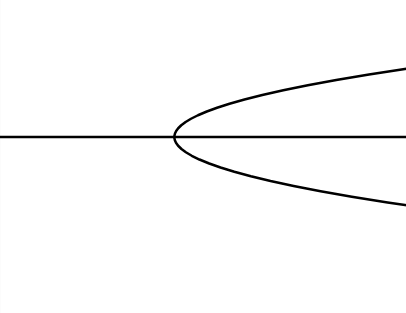
\includegraphics[width=0.48\textwidth]{figures/pitchfork_1.png}\hfill
    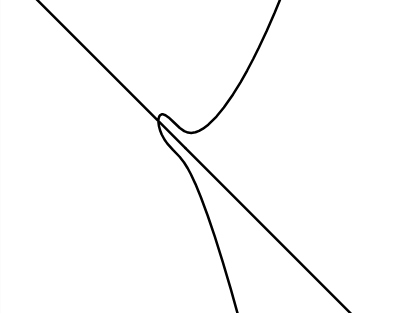
\includegraphics[width=0.48\textwidth]{figures/pitchfork_2.png}
    
    \caption{La pitchfork avant et après la transformation, notez comme cette dernière ne détruit pas l'information "qualitative"}
    \label{fig:pitchfork_globale}
\end{figure}
On peut voir assez rapidement que cette 
relation d'équivalence est pertinente de le 
cadre d'étude de problèmes de bifurcation: 
la matrice $\mathcal{S}$ (en réalité, la germe 
de fonction correspondante...) étant 
inversible, ne change pas l'ensemble 
d'annulation, de plus, si on a un certain 
nombre de solutions en $\lambda_0$, par 
exemple 
$(x_1,\lambda_0)$,...,$(x_n,\lambda_0)$ alors 
cet ensemble va être transporté, via $\phi$ sur 
$(H(x_1,\lambda_0),h(\lambda_0)),\cdots,\\
(H(x_1,\lambda_0),h(\lambda_0))$ et donc,grâce à la structure de $\phi$, elles se trouvent 
sur la même "tranche" $\R^n\times \{h
(\lambda_0)\}$. Si on a une germe 
$g(x,\lambda)$ un peut se demander quelles sont les perturbations qui conservent sa structure, ou plus précisemment, qui ne la font pas changer de classe d'équivalence  pour la relation \ref{GolubEQ}. Soit $p(x,\lambda)$ une germe, considérons la famille $h_t=(g+tp)_{t\in [0,1]}$ 
pour que $p$ soit une perturbation qui conserve la structure, on veut deux choses: d'une part que
\begin{equation*}
    \forall t\in [0,1], h_t\text{ est équivalent à } g 
\end{equation*}  
et d'autre part, on veut que l'équivalence soit lisse. Souvenez vous,la relation d'équivalence  \ref{GolubEQ} exige l'existence de  germes difféomorphismes, ainsi, pour tous $t\in [0,1]$, on aura des germes de difféomorphismes $\phi_t$  et $S_t$, on va naturellement exiger que 
\begin{equation*}
    (x,\lambda,t)\mapsto \phi(x,\lambda,t)\text{ et } (x,\lambda,t)\mapsto S(x,\lambda,t)
\end{equation*} 
définissent des germes lisses
\begin{remarque}
    Le lecteur attentif pourrait se demander comment il est possible de travailler avec un intervalle fixé à priori  alors qu'on travaille avec des germes. Cette imprécision sera levée par lemme de Mather [LEMME]
\end{remarque}

\subsection{détermination finie: généralités}\label{detfin}
C'est le coeur du sujet: on veut 
pouvoir se ramener à l'étude d'un nombre fini de termes du développement de Taylor, comment être sûr qu'on a pas perdu d'information essentielle en tronquant la série ?
Nous introduisons la notion suivante
\begin{definition}
    Si $\mathcal{R}$ est une relation 
    d'équivalence sur $\mathcal{E}(0,\R^n,\R^m)$, on dit que $f$ est $k$-$\mathcal{R}$-\coldef{déterminée} si 
    \begin{equation*}
        \forall g\in \mathcal{E}(0,\R^n,\R^m): j^k g=j^k f, (f,g)\in\mathcal{R}
    \end{equation*}
\end{definition}
Les relations d'équivalences qui nous intéressent seront définies par l'action d'un certain groupe $G$
 \begin{equation*}
    \sim_G : e \sim_Gf \Leftrightarrow \exists g\in G : g\cdot e=f
 \end{equation*}
 Si $G$ agit à droite et $H$ agit à gauche, on définit naturellement l'action de $G\times H$ sur $E$
 \begin{equation*}
    (g,h)\cdot x = g\cdot x \cdot h^{-1}
 \end{equation*}
Le groupe le plus naturel est $d(n)$ l'ensemble des germes de difféomorphismes de $\mathcal{E}(0,\R^n)$, son action sur $\mathcal{E}(0,\R^n,\R^m)$  par composition à droite (resp. à gauche) induit \coldef{l'équivalence droite} (resp. gauche). L'action de $\mathcal{A}=d(n)\times d(m)$ sur $\mathcal{E}(0,\R^n,\R^m)$ induit l'équivalence gauche droite.\\
 On définit le groupe de contact $\mathcal{K}$ comme étant l'ensemble des germes de difféomorphisme des $H\in\mathcal{D}_{n+m}$ telles qu'il existe une $h\in\mathcal{D}_n$ respectant le  diagramme suivant:
\[\begin{tikzcd}
	{(0,\R^{n+m})} & {(0,\R^{n+m})} & \\
	{(0,\R^n)} & {(0,\R^n)} & {\text{avec }\iota(x)=(x,0)}
	\arrow["H", from=1-1, to=1-2]
	\arrow["\pi", from=1-1, to=2-1]
	\arrow["\pi", from=1-2, to=2-2]
	\arrow["\iota", shift left=3, from=2-1, to=1-1]
	\arrow["h", from=2-1, to=2-2]
	\arrow["\iota", shift left=3, from=2-2, to=1-2]
\end{tikzcd}\]
remarquez cela impose que $H$ est de la forme $H(x,y)=(h(x),H_1(x,y))$ en effet 
$H(x,y)=(H_0(x,y),H_1(x,y))$ avec $H_0\in\mathcal{E}^n_{n+m}$, et donc 
\begin{equation*}\label{Structpi}
    \pi\circ H(x,y)= H_0(x,y)=h\circ\pi(x,y)=h(x)
\end{equation*} et que, du fait que 
\begin{equation*}
    H\circ \iota(x)=H(x,0)=(h(x),H_1(x,0))=\iota(h(x))=(h(x),0)
\end{equation*}

On doit avoir que 
\begin{equation}\label{Projo}
    H_1(x,0)=0
\end{equation}
On définit $H\cdot f$ comme étant l'unique germe respectant la condition suivante 
\begin{equation}\label{GraphK}
    (h(x),H\cdot f(h(x)))=H(x,f(x))=(h(x),H_1(x,f(x)))
\end{equation}
Et donc 
\begin{equation}\label{Kequ}
    (H\cdot f)(x)=(H\cdot f)(h (h^{-1}(x)))=H_1(h^{-1}(x),f(h^{-1}(x))) 
\end{equation}


L'équation \ref{GraphK} sert simplement à mettre en évidence le fait que $H$ agit sur $f$ via son graphe. Il est fort possible que vous trouviez dans la littérature une définition différente  de $\mathcal{K}$, montrons qu'elles sont équivalentes
\begin{proposition}\label{MATRIXform}
    $f,g$ sont $\mathcal{K}
    $-équivalentes si et 
    seulement s'il existe 
    $S\in\mathcal{E}(0,\R^n,
    \operatorname{GL_{p}(\R)}) 
    $  et $\phi\in\mathcal{D}_
    {n}$ une  tels que 
    \begin{equation*}
        f\circ \phi= S\cdot g
    \end{equation*}
\end{proposition} 
\begin{preuve}
    Bien sûr, s'il existe $\phi$ et $S$ 
    verifiant la condition de l'énoncé, 
    alors $f,g$ sont $\mathcal{K}
    $-équivalentes. 
    Maintenant supposons qu'elles sont 
    $\mathcal{K}$-équivalentes,via \ref{Kequ}, il existe 
    $H\in\mathcal{D}_{n+p}$ tel que 
    \begin{equation}\label{Proprecr}
        g(h(x))=H_1(x,f(x))
    \end{equation}
    via \ref{Projo}, on sait que 
    $H_1(x,0)=(H_{1,1}(x,0),\cdots,H_{1,n
    +m}(x,0))^T=0$. On applique alors 
    \ref{Hadamard} aux $(H_{1,i})_{1\leq i \leq n+m}$
    \begin{equation*}
        H_{1,i}(x,0)=0\Rightarrow \exists \lambda_{i,1}\cdots \lambda_{i,n}\in\mathcal{E}_{n+m} :H_{1,i}=\sum_{j=1}^m \lambda_{i,j}\pi_j 
    \end{equation*}
    Ainsi, $H_1(x,y)=M(x,y)\cdot y$ avec $M$ une matrice de germe lisses. Le fait que $M$ est inversible découle du fait que $H$ est un difféomorphisme et que sa matrice jacobienne est donnée par 
    \begin{equation*}
        \begin{pmatrix}
        \frac{\partial h}{\partial x} & 0 \\
        \frac{\partial H_1}{\partial x} & \frac{\partial H_1}{\partial y}  \\
        \end{pmatrix} 
    \end{equation*}
    On réécrit \ref{Proprecr} 
    \begin{equation*}
        g(h(x))=M(x,f(x))\cdot f(x)\Leftrightarrow g(x)=M(h^{-1}(x),f(h^{-1}(x)))\cdot f(h^{-1}(x))
    \end{equation*}
    Ce qui permet de conclure
\end{preuve}


 On peut alors reformuler le problème de la façon suivante: $f\in\mathcal{E}(0,\R^n,\R^m)$  est $k$-$E$-déterminée si $\operatorname{orb}_G(f)$ contient les germes ayant le même jet d'ordre $k$ que $f$. On veut un équivalent de ce magnifique résultat de théorie des groupes de Lie 
\begin{theobox}{}{}
    Si $G$ est un groupe de Lie, $M$ une variété lisse, si $G$ agit sur $M$ (par exemple) par la gauche et si $V$ est une sous variété connexe et lisse de $M$ alors 
    \begin{equation*}
        \exists m\in M : V \subseteq G\cdot m \Leftrightarrow \forall v\in V, T_v (G\cdot v) \supseteq T_v (V)\text{ et } \dim T_v (G\cdot v) \text{ est toujours la même }
    \end{equation*}
\end{theobox}
la première condition est assez intuitive: en effet si on prend l'exemple d'une surface $S$ présentant une symétrie de révolution selon un axe, $S^1$ agit sur $S$ (via la rotation autour de l'axe central) et les orbites sont alors des cercles. Ainsi une courbe qui vit dans $S$ sera contenue dans une orbite si c'est un cercle qui entoure l'axe de révolution et on remarque que cela revient à exiger qu'en chaque point, l'espace tangent (ici la droite tangente à la courbe) soit inclus dans celui du cercle entourant l'axe de révolution généré par $S^1$ et ce point. En général, on veut que les points  de $V$ "très proches" de $v$ puissent être atteint par des "petites" $G$-transformations, i.e, si on a pas l'inclusion des espaces tangents, on peut "sortir" de l'orbite. La deuxième condition permet d'éviter les situations "dégénérées" où 
\begin{equation*}
    \Bigl\{G\cdot v | v\in V\Bigr\}  
\end{equation*}
n'est pas une variété. On veut donc une notion "d'espace tangent" pour les orbites induites par les actions décrites ci-dessus.\\


dans \cite{damon1984unfolding}, James damon a obtenu a obtenu des résultats de détermination finie pour une large classe d'équivalences sur les germes les "sous-groupes géométriques de $\mathcal{A}$ et $\mathcal{K}$ . Nous allons passer les prochains paragraphes à en exposer les idées

\subsection{déploiements et espaces tangents}

La notion de déploiement remonte à 
René Thom [SOURCE]. Notez que dans la 
suite, nous supposerons $f\in\mathcal{E}^m_n\cdot \mathcal{M}_n$: ça simplifiera les calculs et ce n'est pas une vraie restriction.
\begin{definition} 
    $G\in\mathcal{E}^{m+d}_{n+d}\cdot \mathcal{M}_{n+d}$ est  \coldef{un déploiement à $d$ paramètres} de $f$
    si elle respecte le diagramme suivant:
    \[\begin{tikzcd}
	{(0,\R^n)} & {(0,\R^m)} \\
	{(0,\R^{n+d})} & {(0,\R^{m+d})} \\
	{(0,\R^d)}
	\arrow["f", from=1-1, to=1-2]
	\arrow["\iota"', from=1-1, to=2-1]
	\arrow["\iota", from=1-2, to=2-2]
	\arrow["G"', from=2-1, to=2-2]
	\arrow["\pi"', from=2-1, to=3-1]
	\arrow["\pi", from=2-2, to=3-1]
    \end{tikzcd}\]
    des calculs similaires à \ref{Structpi} permettent de voir que cela impose à $G$ d'être de la forme $G(x,u)=(G_1(x,u),u)$ et 
    $G_1(\cdot,0)=f$
    On pose $\mathcal{U}_d(f)$ l'ensemble des déploiements à $d$ paramètres de $f$.
\end{definition}

\begin{remarque}
    dans la littérature, la notion de déploiement et parfois interchangée avec la notion de \coldef{déformation}. Une déformation $F$ de $f$ est simplement une germe de $\mathcal{E}^{m}_{n+d}$ telle que $F(\cdot,0)=f$. En quelque sorte, le déploiement "mémorise" le paramètre mais pas la déformation.
\end{remarque}

\begin{definition}
    Soit $V\subseteq \mathcal{E}^m_n\cdot \mathcal{M}_n$  et $v\in V$ une \coldef{famille à $d$-paramètres}  $G$   \coldef{ à travers} $v$ \coldef{dans $V$} est un élément de  $\mathcal{U}_d(v)$ tel qu'il existe un représentant de  $G_1$, $\tilde{G}_1$ et un voisinage de 0 $U$ tel que $[\tilde{G_1}(u,\cdot)]\in V$ si $u\in U$. L'ensemble de tel déploiements sera noté $\mathcal{U}_d(v,V)$
\end{definition}

\begin{exemple}
    Si $V=\mathcal{M}^2_1$ et $v(x)=x^3$, alors 
    \begin{equation*}
        G_1(x,u)=x^3+ux^2
    \end{equation*}
    est une famille à 1 paramètres à travers $v$ dans $V$. Mais par exemple 
    \begin{equation*}
        G_2(x,u)=x^3+ux
    \end{equation*}
    ne l'est pas.
\end{exemple}
On va s'intéresser particulièrement aux famille à 1 seul paramètre, c'est à dire les \coldef{chemin lisses} dans une sous "variété"  $V$ de $\mathcal{E}^n_m$.


Rappelons que si $M$ est $N$ sont des variétés lisses et si $f\in C^{\infty}(M,N)$ alors l'ensemble des champs de vecteurs lisses \coldef{le long} de $f$, $\mathcal{V}(f)$ est donné par l'ensemble des $\xi: M\rightarrow TN$
respectant le diagramme suivant: 

\[\begin{tikzcd}
	TM & TN \\
	M & N
	\arrow["Tf", from=1-1, to=1-2]
	\arrow["\pi"', from=1-1, to=2-1]
	\arrow["\pi", from=1-2, to=2-2]
	\arrow["\xi", from=2-1, to=1-2]
	\arrow["f", from=2-1, to=2-2]
\end{tikzcd}\]
On remarque alors que
\begin{equation*}
    \mathcal{V}(f)=\Gamma f^{*} TN
\end{equation*}
Considérons alors le faisceau (c.f remarque \ref{remsheaf} )
des sections locales lisses 
$\Gamma(\cdot,TM)$, l'ensemble des germes de champ de vecteurs en un point $x\in M$ est simplement $\Gamma(\cdot,TM)_x$ et l'ensemble des germes de champ de vecteurs le long de $f$ en $x$ est $\Gamma(\cdot, f^{*}T\R^m)_{x}$

Maintenant, si $f\in\mathcal{E}^m_n$, on entend par $\mathcal{V}(f)$ la germe en $0$ des champs de vecteurs le long d'un représentant de $f$.
du fait que $T \R^m\cong \R^{2m} $, on vérifie facilement que 
\begin{equation*}
    \mathcal{V}(f)=
    \biggr>\frac{\partial }{\partial y_1},\cdots, \frac{\partial  }{\partial y_m}  \biggl<_{\mathcal{E}_n}
\end{equation*}



\begin{definition}
    Soit $V\subseteq \mathcal{E}^m_n$ et $f\in V$ on définit \coldef{l'espace tangent de $v$}
    comme 
    \begin{equation*}
        T_f V =\left\{\frac{\partial G}{\partial u}(0) \biggr| G\in\mathcal{U}_1(f,V) \right\}
    \end{equation*}
\end{definition}

On vérifie aussi facilement que les éléments de $T_f V$ sont bien des vecteurs le long de $f$.

\begin{proposition}
    \begin{equation*}
        T_f \mathcal{K}\cdot f=\cdots
    \end{equation*}
\end{proposition}
\begin{preuve}
    Soit $G\in\mathcal{U}_1(f,\mathcal{K}\cdot f)$, c'est à dire une germe de le forme
    \begin{equation*}
        G(x,u)= (H_u\cdot f(x),u)\text{ avec $H_u\in \mathcal{K}$}
    \end{equation*}
    On peut supposer sans perte de généralité que $H_{0}=\operatorname{Id}$. Via \ref{MATRIXform} et \ref{GraphK}, on écrit 
    \begin{equation*}
        H_u\cdot f(x)=M_u(h_u^{-1}(x),f(h_{u}^{-1}(x)))\cdot f(h_u^{-1}(x))
    \end{equation*}
    Et on calcule alors 
    \begin{equation}
        \frac{\partial G}{\partial u}(0)= 
    \end{equation}

\end{preuve}

\todo{Un théorème de détermination finie}\\
\todo{Le groupe de montaldi}\\
\todo{Classification explicite}\\
\todomaybe{Notion de sous-groupe géométrique}
\newpage
\end{document}